% \documentclass{article}
% \documentclass{book}
\documentclass{report} % Chọn cỡ chữ
\usepackage{Start}
\begin{document} % Bắt đầu
%!%%%%%%%%%%%%%%%%%%%%%%%%%%%%
%!%%%%%%%%%%%%%%%%%%%%%%%%%%%%
%!%%%%%%%%%%%%%%%%%%%%%%%%%%%%
%!%%%%%%%%%%%%%%%%%%%%%%%%%%%%
%!%%%%%%%%%%%%%%%%%%%%%%%%%%%%
%!%%%%%%%%%%%%%%%%%%%%%%%%%%%%
%!%%%%%%%%%%%%%%%%%%%%%%%%%%%%
%!%%%%%%%%%%%%%%%%%%%%%%%%%%%%
%!%%%%%%%%%%%%%%%%%%%%%%%%%%%%
%!%%%%%%%%%%%%%%%%%%%%%%%%%%%%
%!%%%%%%%%%%%%%%%%%%%%%%%%%%%%
%!%%%%%%%%%%%%%%%%%%%%%%%%%%%%
%!%%%%%%%%%%%%%%%%%%%%%%%%%%%%
%!%%%%%%%%%%%%%%%%%%%%%%%%%%%%
%!%%%%%%%%%%%%%%%%%%%%%%%%%%%%
%!%%%%%%%%%%%%%%%%%%%%%%%%%%%%
%!%%%%%%%%%%%%%%%%%%%%%%%%%%%%
%!%%%%%%%%%%%%%%%%%%%%%%%%%%%%
%!%%%%%%%%%%%%%%%%%%%%%%%%%%%%
%!%%%%%%%%%%%%%%%%%%%%%%%%%%%%
%!%%%%%%%%%%%%%%%%%%%%%%%%%%%%
%!%%%%%%%%%%%%%%%%%%%%%%%%%%%%
%!%%%%%%%%%%%%%%%%%%%%%%%%%%%%
%!%%%%%%%%%%%%%%%%%%%%%%%%%%%%
%!%%%%%%%%%%%%%%%%%%%%%%%%%%%%
%!%%%%%%%%%%%%%%%%%%%%%%%%%%%%
%# Phần đầu
%#%%%%%%%%%%%%%%%%%%%%%%%%%%%%
% \begin{titlepage}

    % Vẽ hình chữ nhật
    
    \begin{tikzpicture}[remember picture, overlay]\draw [line width = 3pt]($ (current page.north west) + (3.0cm, - 2.5cm)$)rectangle($ (current page.south east) + (- 2.5cm, 2.5cm)$);\draw [line width = 0.5pt]($ (current page.north west) + (3.1cm, - 2.6cm)$)rectangle($ (current page.south east) + (- 2.6cm, 2.6cm)$);\end{tikzpicture}
    
    \begin{center}
    
    \vspace{- 0.4cm}
    
    \textbf{ĐẠI HỌC BÁCH KHOA HÀ NỘI} \\
    
    \textbf{VIỆN TOÁN ỨNG DỤNG VÀ TIN HỌC} \\
    
    \textbf{******}
    
    \vspace{0.8cm}
    
    \begin{figure}[H]
    
    \centering
    
    
\includegraphics[scale = 0.5]{pictures/_hust/main.png}
    
    \end{figure}
    
    \vspace{0.7cm}
    
    \textbf{\fontsize{16pt}{30pt}\selectfont {BÁO CÁO ĐỒ ÁN II}}
    
    \vspace{1cm}
    
    \textbf{\fontsize{16pt}{30pt}\selectfont {ĐỀ TÀI:}} \\
    
    \textbf{\fontsize{20pt}{24pt}\selectfont {Sử dụng thiết kế hướng miền \\ xây dựng kiến trúc vi dịch vụ cho \\ bài toán hóa đơn điện tử}} \\
    
    \end{center}
    
    \vspace{0.3cm}
    
    \begin{center}
    
    \textbf{\fontsize{10pt}{24pt}\selectfont {Chuyên ngành: Toán Tin}}
    
    \end{center}
    
    \vspace{0.7cm}
    
    \hspace{3cm}\begin{minipage}{0.7\textwidth}
    
    \begin{tabular}{l l l}
    
    \textbf{\fontsize{10pt}{24pt}\selectfont {Giảng viên hướng dẫn}} & \textbf{\fontsize{10pt}{24pt}\selectfont {TS. Vũ Thành Nam}} \\
    
    \textbf{\fontsize{10pt}{24pt}\selectfont {Sinh viên thực hiện}} & \textbf{\fontsize{10pt}{24pt}\selectfont {Vũ Văn Nghĩa}} \\
    
    \textbf{\fontsize{10pt}{24pt}\selectfont {Mã số sinh viên}} & \textbf{\fontsize{10pt}{24pt}\selectfont {20206205}} \\
    
    \textbf{\fontsize{10pt}{24pt}\selectfont {Lớp}} & \textbf{\fontsize{10pt}{24pt}\selectfont {Toán Tin 02 - K65}} \\
    
    \end{tabular}
    
    \end{minipage}
    
    \vfill
    
    \begin{center}
    
    \textbf{Hà Nội, \the\year}
    
    % \textbf{Hà Nội, \the\month~/~\the\year}
    
    % \textbf{Hà Nội, \the\month~-~\the\year}
    
    \end{center}
    
    \end{titlepage}
    
    
% \begin{titlepage}

    % Vẽ hình chữ nhật
    
    \begin{tikzpicture}[remember picture, overlay]\draw [line width = 3pt]($ (current page.north west) + (3.0cm, - 2.5cm)$)rectangle($ (current page.south east) + (- 2.5cm, 2.5cm)$);\draw [line width = 0.5pt]($ (current page.north west) + (3.1cm, - 2.6cm)$)rectangle($ (current page.south east) + (- 2.6cm, 2.6cm)$);\end{tikzpicture}
    
    \begin{center}
    
    \vspace{- 0.4cm}
    
    \textbf{ĐẠI HỌC BÁCH KHOA HÀ NỘI} \\
    
    \textbf{VIỆN TOÁN ỨNG DỤNG VÀ TIN HỌC} \\
    
    \textbf{******}
    
    \vspace{0.8cm}
    
    \begin{figure}[H]
    
    \centering
    
    
\includegraphics[scale = 0.5]{pictures/_hust/main.png}
    
    \end{figure}
    
    \vspace{0.7cm}
    
    \textbf{\fontsize{16pt}{30pt}\selectfont {BÁO CÁO ĐỒ ÁN II}}
    
    \vspace{1cm}
    
    \textbf{\fontsize{16pt}{30pt}\selectfont {ĐỀ TÀI:}} \\
    
    \textbf{\fontsize{20pt}{24pt}\selectfont {Sử dụng thiết kế hướng miền \\ xây dựng kiến trúc vi dịch vụ cho \\ bài toán hóa đơn điện tử}} \\
    
    \end{center}
    
    \vspace{0.3cm}
    
    \begin{center}
    
    \textbf{\fontsize{10pt}{24pt}\selectfont {Chuyên ngành: Toán Tin}}
    
    \end{center}
    
    \vspace{0.7cm}
    
    \hspace{3cm}\begin{minipage}{0.7\textwidth}
    
    \begin{tabular}{l l l}
    
    \textbf{\fontsize{10pt}{24pt}\selectfont {Giảng viên hướng dẫn}} & \textbf{\fontsize{10pt}{24pt}\selectfont {TS. Vũ Thành Nam}} \\
    
    \textbf{\fontsize{10pt}{24pt}\selectfont {Sinh viên thực hiện}} & \textbf{\fontsize{10pt}{24pt}\selectfont {Vũ Văn Nghĩa}} \\
    
    \textbf{\fontsize{10pt}{24pt}\selectfont {Mã số sinh viên}} & \textbf{\fontsize{10pt}{24pt}\selectfont {20206205}} \\
    
    \textbf{\fontsize{10pt}{24pt}\selectfont {Lớp}} & \textbf{\fontsize{10pt}{24pt}\selectfont {Toán Tin 02 - K65}} \\
    
    \end{tabular}
    
    \end{minipage}
    
    \vfill
    
    \begin{center}
    
    \textbf{Hà Nội, \the\year}
    
    % \textbf{Hà Nội, \the\month~/~\the\year}
    
    % \textbf{Hà Nội, \the\month~-~\the\year}
    
    \end{center}
    
    \end{titlepage}
    
    
% \begin{center}

    {\bfseries NHẬN XÉT CỦA GIẢNG VIÊN HƯỚNG DẪN}
    
    \end{center}
    
    \begin{enumerate}
    
    \item Mục đích và nội dung của đồ án:
    
    \vspace{20ex}
    
    \item Kết quả đạt được:
    
    \vspace{20ex}
    
    \item Ý thức làm việc của sinh viên:
    
    \vspace{20ex}
    
    \end{enumerate}
    
    \hspace{0.4\textwidth}\begin{minipage}{0.5\textwidth}
    
    \noindent\begin{center}
    
    \textit{Hà Nội, \today} \\
    
    \textbf{Giảng viên hướng dẫn} \\
    
    \textit{(Ký và ghi rõ họ tên)}
    
    \vspace{2cm}
    
    \textbf{TS. Vũ Thành Nam}
    
    \end{center}
    
    \end{minipage}
    
    \pagestyle{empty}
    
    
% 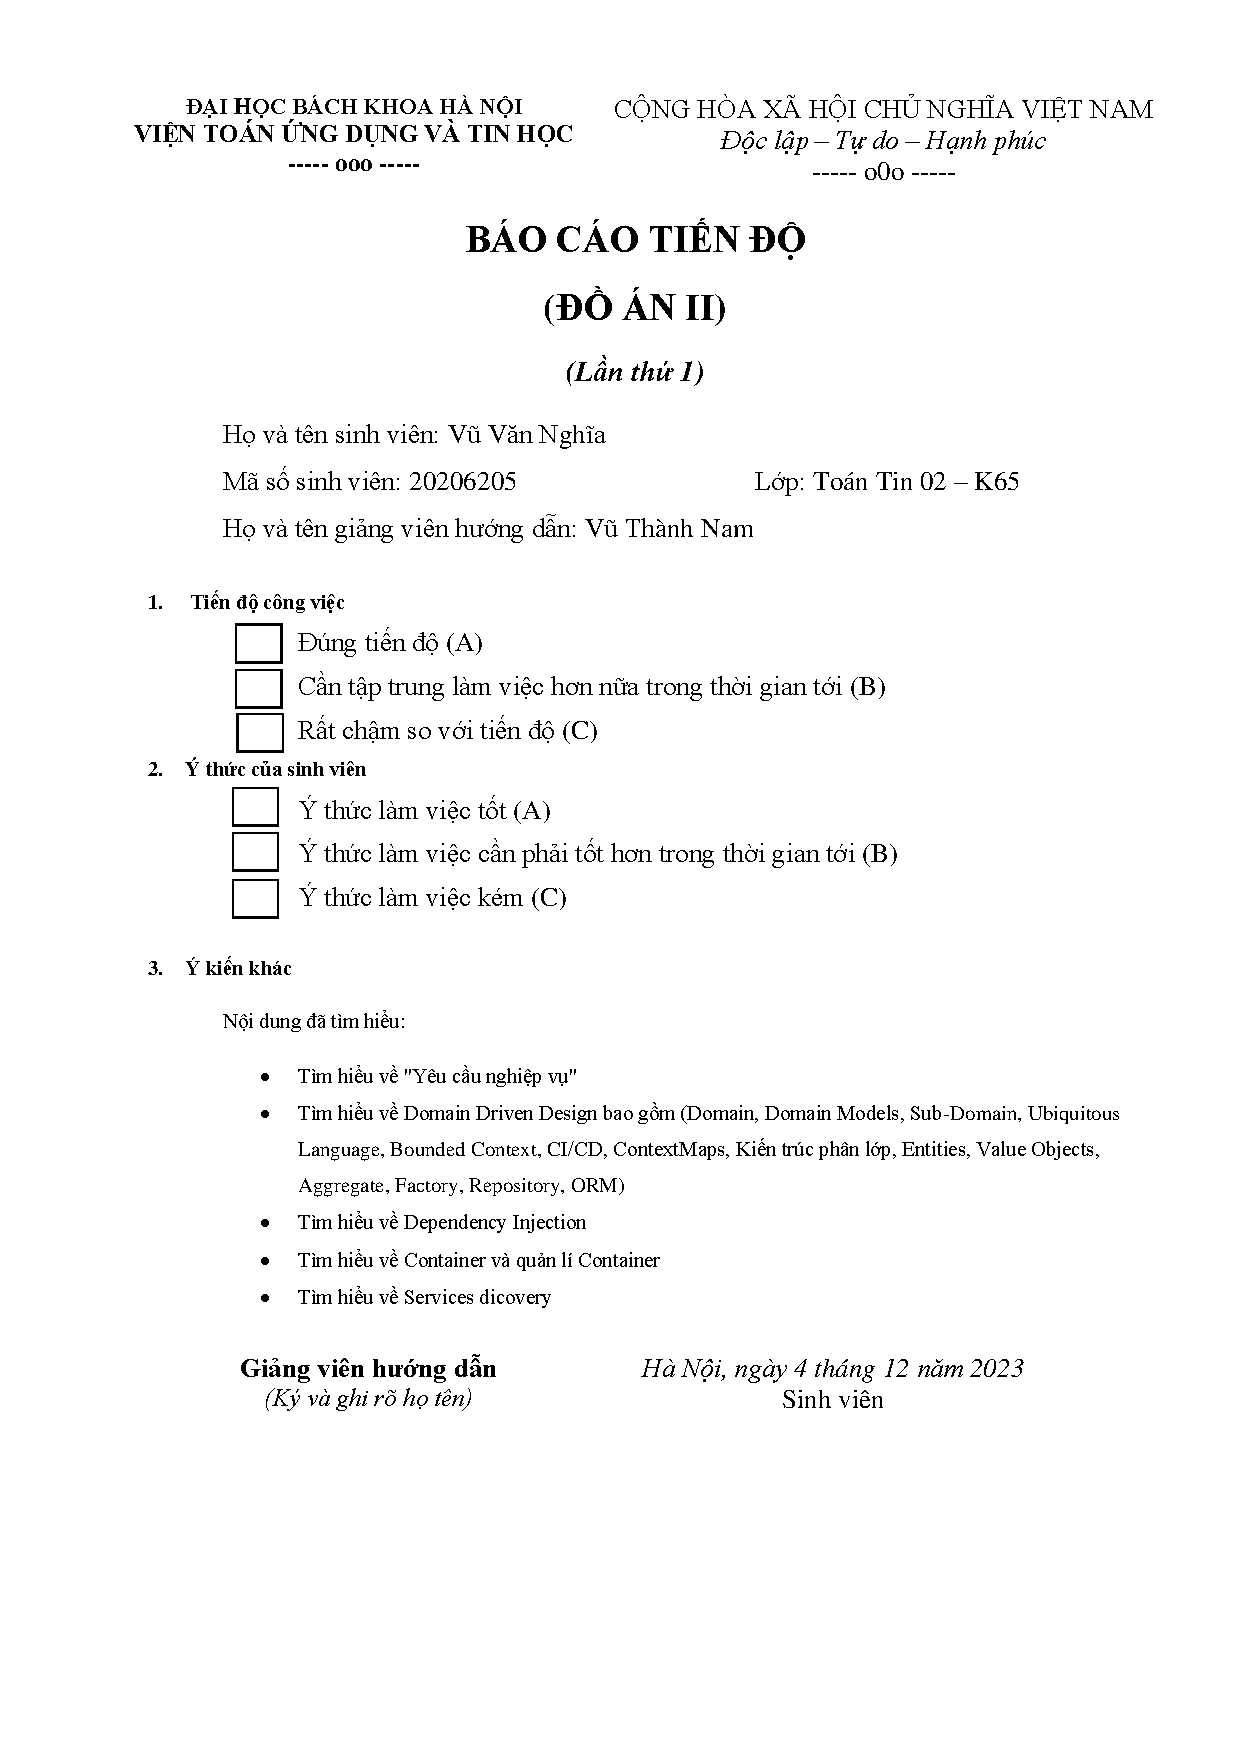
\includepdf[pages = -]{contents/bao_cao_tien_do/lan_1.pdf}
% 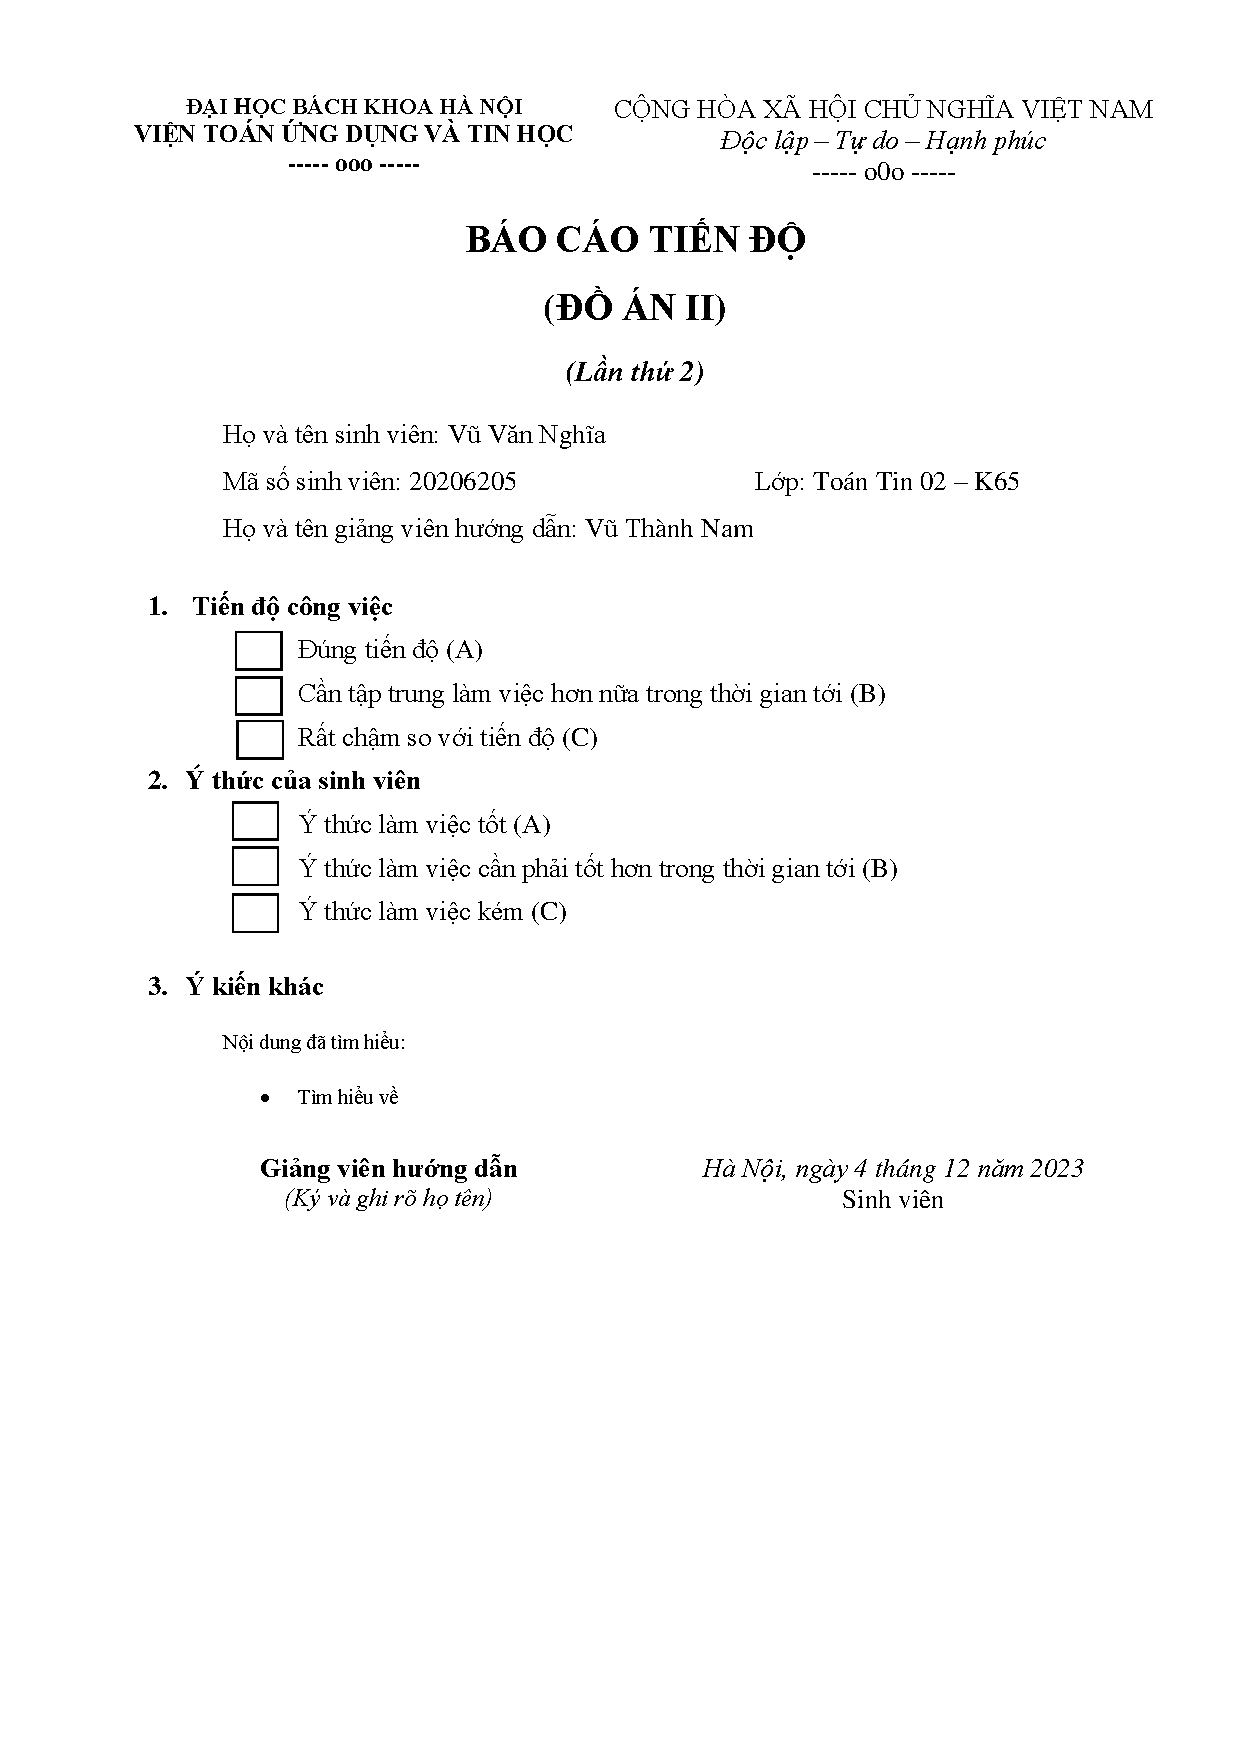
\includepdf[pages = -]{contents/bao_cao_tien_do/lan_2.pdf}
% \renewcommand*\contentsname{\centering MỤC LỤC}

\tableofcontents

\setcounter{page}{0}


% \chapter*{\centering LỜI CẢM ƠN}

\addcontentsline{toc}{chapter}{LỜI CẢM ƠN}

Trước hết, em xin gửi lời cảm ơn chân thành và sâu sắc đến TS. Vũ Thành Nam, người thầy đã tận tình hỗ trợ và hướng dẫn em suốt thời gian thực hiện đồ án. Những kiến thức và kinh nghiệm mà em đã tiếp thu được trong quá trình này sẽ đóng góp quan trọng vào sự phát triển và thành công của em trong tương lai. Em xin gửi lời chúc sức khỏe tốt nhất đến thầy, hy vọng thầy luôn dồi dào sức khỏe, đam mê và nhiệt huyết trong công việc giảng dạy.

Em cũng xin gửi lời cảm ơn tới các thầy cô giảng viên trong \emph{"Khoa Toán - Tin"} đã tận tình truyền đạt những kiến thức quý báu cho em. Những kiến thức này không chỉ giúp em phát triển về mặt tri thức mà còn nuôi dưỡng kỹ năng và đam mê trong quá trình học tập và nghiên cứu.

Trong quá trình hoàn thành bài báo cáo đồ án này không tránh khỏi những thiếu sót. Vì vậy, em mong nhận được sự giúp đỡ và ý kiến đóng góp chân thành từ các thầy cô để em có thể cải thiện một cách tốt nhất.

\emph{Em xin chân thành cảm ơn!}

\vspace{0.7cm}

\hspace{0.4\textwidth}\begin{minipage}{0.5\textwidth}

\noindent\begin{center}

\textit{Hà Nội, \today} \\

\vspace{0.5cm}

\textbf{Tác giả} \\

\vspace{0.5cm}

\textbf{Vũ Văn Nghĩa}

\end{center}

\end{minipage}
% \chapter*{\centering DANH SÁCH BẢNG}

\addcontentsline{toc}{chapter}{DANH SÁCH BẢNG}

\makeatletter

\renewcommand\listoftables{

\@starttoc{lot}

}

\makeatother

\listoftables
% \chapter*{\centering DANH SÁCH HÌNH ẢNH}

\addcontentsline{toc}{chapter}{DANH SÁCH HÌNH ẢNH}

\makeatletter

\renewcommand\listoffigures{

\@starttoc{lof}

}

\makeatother

\listoffigures
% %%%%%%%%%%%%%%%%%%%%%%%%%%%%%%

%%%%%%%%%%%%%%%%%%%%%%%%%%%%%%

\chapter*{\centering DANH SÁCH CÁC CỤM TỪ VIẾT TẮT}

\addcontentsline{toc}{chapter}{DANH SÁCH CÁC CỤM TỪ VIẾT TẮT}

% @sau

% @sau

% @sau

% @sau

% @sau

% @sau

% @sau

% @sau

% @sau

% @sau

% @sau

% @sau

% @sau

% @sau

% @sau

% @sau

% @sau

% @sau

% @sau

% @sau

% @sau

% @sau

% @sau

% @sau

% @sau

% @sau

% @sau

% @sau

% @sau

% @sau

\begin{table}[h]

\centering

\begin{tabular}{|c|c|c|c|}

\hline

STT & Từ viết tắt & Từ viết đầy đủ & Mô tả \\

\hline

Dong1 & Dong1 & Cot1 & Cot2 \\

\hline

Dong2 & Dong2 & Cot1 & Cot2 \\

\hline

\end{tabular}

\end{table}

% API; Application Programming Interface; Giao diện lập trình ứng dụng

% CI/CD; Continuous Integration (CI) and Continuous Delivery (CD) ; Quá trình tích hợp và chuyển giao liên tục

% thiết kế hướng miền ; thiết kế hướng miền; Kỹ thuật thiết kế theo hướng miền

% DI; Dependency Injection; Cơ chế tiêm sự phụ thuộc giữa các đối tượng

% HTTP; Hypertext Transfer Protocol; Giao thức truyền tải siêu văn bản

% JSON; JavaScript Object Notation; Một kiểu dữ liệu mở rộng của JavaScript

% ORM; Object Relational Mapping; Một kỹ thuật ánh xạ các đối tượng lập trình với từng bảng trong CSDL quan hệ

% Cơ sở dữ liệu ; CSDL ;

% Tạo (Create), Đọc (Read), Sửa (Update), Xóa (Delete) ; CRUD ;

% Kubernetes ; K8s ; kubernetes

% Số điện thoại ; SĐT ;

% UML

% MVC; Model View Controller; Một mẫu thiết kế ứng dụng

% SQL

SOA; Service Oriented Architecture; Kiến trúc hướng dịch vụ

SOAP; Simple Object Access Protocol; Một giao thức để truy cập dịch vụ web

SPA; Single Page Application; Kiểu ứng dụng một trang

REST; Representational State Transfer; Một tiêu chuẩn thiết kế các API sử dụng cho các dịch vụ web

URL; Uniform Resource Locator ; Địa chỉ định vị tài nguyên trên Internet

XML; Extensible Markup Language; Ngôn ngữ đánh dấu mở rộng

% TCT ; TCT ;

Người nộp thuế ; NNT ;

Mã số thuế ; MST ;

Hóa đơn điện tử ; HĐĐT ;

Cơ quan thuế ; CQT ;

Công nghệ thông tin ; CNTT ;

%%%%%%%%%%%%%%%%%%%%%%%%%%%%%%
% \chapter*{\centering DANH SÁCH CÁC THUẬT NGỮ}

\addcontentsline{toc}{chapter}{DANH SÁCH CÁC THUẬT NGỮ}

% @sau

% @sau

% @sau

% @sau

% @sau

% @sau

% @sau

% @sau

% @sau

% @sau

% @sau

% @sau

% @sau

% @sau

% @sau

% @sau

% @sau

% @sau

% @sau

% @sau

% @sau

% @sau

% @sau

% @sau

% @sau

% @sau

% @sau

% @sau

\begin{table}[h]

\centering

\begin{tabular}{|c|c|c|}

\hline

STT & Tiếng Anh & Tiếng Việt \\

\hline

Dong1 & Dong1 & Cot2 \\

\hline

Dong2 & Dong2 & Cot2 \\

\hline

\end{tabular}

\end{table}

% kiến trúc nguyên khối, kiến trúc nguyên khối

% kiến trúc nguyên khối, kiến trúc nguyên khối

% kiến trúc vi dịch, kiến trúc vi dịch

% kiến trúc vi dịch, kiến trúc vi dịch

% kiến trúc vi dịch, kiến trúc vi dịch

% kiến trúc vi dịch, kiến trúc vi dịch

% thiết kế hướng miền, thiết kế hướng miền

% thiết kế hướng miền, thiết kế hướng miền

1 thiết kế hướng miền

Thiết kế hướng lĩnh vực

2 Domain (không dịch)

3 Abstraction Trừu tượng

4 chuyên gia ngành
%#%%%%%%%%%%%%%%%%%%%%%%%%%%%%
%%%%%%%%%%%%%%%%%%%%%%%%%%%%%%
%%%%%%%%%%%%%%%%%%%%%%%%%%%%%%
%%%%%%%%%%%%%%%%%%%%%%%%%%%%%%
%%%%%%%%%%%%%%%%%%%%%%%%%%%%%%
%%%%%%%%%%%%%%%%%%%%%%%%%%%%%%
%%%%%%%%%%%%%%%%%%%%%%%%%%%%%%
%%%%%%%%%%%%%%%%%%%%%%%%%%%%%%
%%%%%%%%%%%%%%%%%%%%%%%%%%%%%%
%%%%%%%%%%%%%%%%%%%%%%%%%%%%%%
%# Phần mở đầu đồ án nào cũng có
%#%%%%%%%%%%%%%%%%%%%%%%%%%%%%
% \chapter*{\centering MỞ ĐẦU}
% \addcontentsline{toc}{chapter}{MỞ ĐẦU}
% \section*{Lý do chọn đề tài}
% Trong quá trình hoạt động kinh doanh, doanh nghiệp có nhu cầu chuyển đổi mô hình kinh doanh linh hoạt để có thể tồn tại và phát triển khi thị trường thay đổi. Từ đó, đáp ứng nhu cầu của khách hàng, mang lại ưu thế cạnh tranh so với các đối thủ.

Trong những năm gần đây, việc áp dụng kiến trúc vi dịch vụ ngày càng phổ biến, đem lại nhiều lợi ích như tách các nghiệp vụ kinh doanh thành các dịch vụ nhỏ độc lập, tăng tính linh hoạt và khả năng chống chịu sự cố của hệ thống.

Kiến trúc vi dịch vụ hỗ trợ doanh nghiệp chuyển đổi nhanh chóng để đáp ứng nhu cầu của mô hình kinh doanh và mong đợi của khách hàng. Tuy nhiên, để xây dựng được kiến trúc vi dịch vụ tốt, cần phải tạo ra các dịch vụ nhỏ phù hợp và duy trì tính độc lập. Trong đồ án này, em sử dụng thiết kế hướng miền để phân tích và xây dựng kiến trúc vi dịch vụ.

Theo quy định của Nghị định 123/2020/NĐ - CP, tất cả các doanh nghiệp, tổ chức và hộ kinh doanh đều bắt buộc phải sử dụng hóa điện tử. Vì vậy, nhu cầu sử dụng và xử lý hóa đơn điện tử trở nên rất lớn. Do đó trong đồ án này, em chọn chủ đề \emph{"Sử dụng thiết kế hướng miền xây dựng kiến trúc vi dịch vụ cho bài toán hóa đơn điện tử"}. Chủ đề này là một xu hướng quan trọng trong phát triển phần mềm và mang lại nhiều lợi ích trong việc cải thiện quá trình quản lý hóa đơn điện tử.
% \section*{Đối tượng và phạm vi nghiên cứu}
% \begin{itemize}

\item \textbf{Đối tượng nghiên cứu:} Kiến trúc vi dịch vụ

\item \textbf{Phạm vi nghiên cứu:} Tập trung vào tìm hiểu thiết kế hướng miền xây dựng kiến trúc vi dịch vụ cho bài toán hóa đơn điện tử.

\end{itemize}


% \section*{Tóm tắt nội dung đồ án}
% Báo cáo đồ án này được tổ chức thành các phần chính sau:

\begin{itemize}

    \item \textbf{Chương 1: xxxxxxxxxxxxxxxxx}

    \begin{quote}
    
        xxxxxxxxxxxxxxxxx
    
    \end{quote}  
    \item \textbf{Chương 1: xxxxxxxxxxxxxxxxx}
    
    \begin{quote}
    
        xxxxxxxxxxxxxxxxx
    
    \end{quote}  
    \item \textbf{Chương 1: xxxxxxxxxxxxxxxxx}
    
    \begin{quote}
    
        xxxxxxxxxxxxxxxxx
    
    \end{quote}  

\end{itemize}

%@ Thêm các mục nhỏ như:

%@ Thêm các mục nhỏ như:

%@ Thêm các mục nhỏ như:

%@ Thêm các mục nhỏ như:

%@ Thêm các mục nhỏ như:

%@ Thêm các mục nhỏ như:

%@ Thêm các mục nhỏ như:

%@ Thêm các mục nhỏ như:

%@ Thêm các mục nhỏ như:

%@ Thêm các mục nhỏ như:

%@ Thêm các mục nhỏ như:

%@ Thêm các mục nhỏ như:

%@ Thêm các mục nhỏ như:

% Luận văn được tổ chức thành các phần chính sau:

% Mở đầu: Trình bày tổng quan về đề tài

% Chương 1: Trình bày cách thức phát triển phần mềm theo kiến trúc kiến trúc vi dịch vụ .

% Trong chương này, luận văn tập trung làm rõ các nội dung:

% - Sơ lược về một số hướng kiến trúc phần mềm truyền thống như kiến trúc nguyên

% khối, kiến trúc hướng dịch vụ, công nghệ ESB

% - Tổng quan về kiến trúc kiến trúc vi dịch vụ : sự ra đời, đặc điểm của kiến trúc vi dịch vụ

% - Các mẫu thiết kế quan trọng được sử dụng trong kiến trúc vi dịch vụ

% - Một số nguyên tắc thiết kế kiến trúc vi dịch vụ

% Chương 2: Trình bày hướng xây dựng ứng dụng web sử dụng micro - frontends.

% Trong chương này, luận văn tập trung làm rõ các nội dung:

% - Sơ lược về một số mô hình phát triển web như mô hình web tĩnh, mô hình web

% động, mô hình web theo hướng SPA

% - Sự ra đời của kiến trúc micro - frontends

% - Các cơ chế tích hợp micro - frontends được thảo luận như: tích hợp theo hướng

% “build - time”, tích hợp theo hướng “run - time”, cách thức điều hướng và giao tiếp

% giữa các micro - frontends

% Chương 3: Trình bày cách thức xây dựng một ứng dụng thử nghiệm sử dụng kiến

% trúc kiến trúc vi dịch vụ, micro - frontends. Một số nội dung chính trong quá trình thực nghiệm

% được làm rõ bao gồm:

% 3

% - Áp dụng phương pháp thiết kế hướng miền để phân hoạch, thiết kế chương trình

% - Thiết kế và cài đặt tầng dịch vụ theo hướng kiến trúc vi dịch vụ, sử dụng các công

% nghệ trên nền tảng Java như Spring Boot, Spring Cloud

% - Thiết kế và cài đặt tầng giao diện theo hướng micro - frontends, sử dụng các công

% nghệ như Single - SPA, Angular, ReactJS

% - Một số kỹ thuật kiểm thử kiến trúc vi dịch vụ cũng được thảo luận như kiểm thử đơn

% vị, kiểm thử tích hợp và kiểm thử mức giao diện

% - Cách thức triển khai ứng dụng sử dụng Docker

% Phần kết luận: Tổng kết, đánh giá kết quả thu được của quá trình nghiên cứu cũng

% như các ưu nhược điểm, các hạn chế và hướng phát triển tương lai.
% \end{document}
%#%%%%%%%%%%%%%%%%%%%%%%%%%%%%
%%%%%%%%%%%%%%%%%%%%%%%%%%%%%%
%%%%%%%%%%%%%%%%%%%%%%%%%%%%%%
%%%%%%%%%%%%%%%%%%%%%%%%%%%%%%
%%%%%%%%%%%%%%%%%%%%%%%%%%%%%%
%%%%%%%%%%%%%%%%%%%%%%%%%%%%%%
%%%%%%%%%%%%%%%%%%%%%%%%%%%%%%
%%%%%%%%%%%%%%%%%%%%%%%%%%%%%%
%%%%%%%%%%%%%%%%%%%%%%%%%%%%%%
%%%%%%%%%%%%%%%%%%%%%%%%%%%%%%
%# Bài toán hóa đơn điện tử
%#%%%%%%%%%%%%%%%%%%%%%%%%%%%%
% \chapter{Bài toán hóa đơn điện tử}
% \section{Các khái niệm và căn cứ pháp lý}
% \section{Yêu cầu nghiệp vụ}
% \section{Phân tích sơ đồ Use Case}
% \end{document}
%#%%%%%%%%%%%%%%%%%%%%%%%%%%%%
%%%%%%%%%%%%%%%%%%%%%%%%%%%%%%
%%%%%%%%%%%%%%%%%%%%%%%%%%%%%%
%%%%%%%%%%%%%%%%%%%%%%%%%%%%%%
%%%%%%%%%%%%%%%%%%%%%%%%%%%%%%
%%%%%%%%%%%%%%%%%%%%%%%%%%%%%%
%%%%%%%%%%%%%%%%%%%%%%%%%%%%%%
%%%%%%%%%%%%%%%%%%%%%%%%%%%%%%
%%%%%%%%%%%%%%%%%%%%%%%%%%%%%%
%%%%%%%%%%%%%%%%%%%%%%%%%%%%%%
%# Giới thiệu về kiến trúc vi dịch vụ
%#%%%%%%%%%%%%%%%%%%%%%%%%%%%%
% \chapter{Giới thiệu về kiến trúc vi dịch vụ}
% \section{Kiến trúc nguyên khối (Monolithic architecture)}
% \section{Kiến trúc vi dịch vụ (Microservices architecture)}
% \section{Một số đặc điểm và ưu điểm của kiến trúc vi dịch vụ}
% \section{Một số nhược điểm và thách thức của kiến trúc vi dịch vụ}
% \end{document}
%#%%%%%%%%%%%%%%%%%%%%%%%%%%%%
%%%%%%%%%%%%%%%%%%%%%%%%%%%%%%
%%%%%%%%%%%%%%%%%%%%%%%%%%%%%%
%%%%%%%%%%%%%%%%%%%%%%%%%%%%%%
%%%%%%%%%%%%%%%%%%%%%%%%%%%%%%
%%%%%%%%%%%%%%%%%%%%%%%%%%%%%%
%%%%%%%%%%%%%%%%%%%%%%%%%%%%%%
%%%%%%%%%%%%%%%%%%%%%%%%%%%%%%
%%%%%%%%%%%%%%%%%%%%%%%%%%%%%%
%%%%%%%%%%%%%%%%%%%%%%%%%%%%%%
%# Thiết kế hướng miền
%#%%%%%%%%%%%%%%%%%%%%%%%%%%%%
\chapter{Thiết kế hướng miền}

\section{Đôi nét về thiết kế hướng miền (Domain Driven Design)}
% Thiết kế hướng miền được   \emph{ Eric Evans}     giới thiệu trong cuốn sách \emph{"Domain Driven Design: Tackling Complexity in the Heart of Software"}. \emph{Thiết kế hướng miền (Domain Driven Design)} là một hướng tiếp cận thiết kế phần mềm tập trung vào việc hiểu rõ và mô hình hóa lĩnh vực kinh doanh của một tổ chức. Thiết kế hướng miền nhấn mạnh việc sử dụng lĩnh vực nghiệp vụ kinh doanh để thảo luận và đề xuất giải pháp đáp ứng nhu cầu.

Với nhiều phần mềm được thiết kế không tốt, phần xử lý các công việc không liên quan đến vấn đề nghiệp vụ kinh doanh như truy cập tập tin, hạ tầng mạng, cơ sở dữ liệu, \dots được lập trình trong đối tượng nghiệp vụ kinh doanh. Cách này có ưu điểm giúp tốc độ hoàn thiện phần mềm nhanh. Tuy nhiên, cách này làm dự án bị mất đi tính hướng đối tượng khó thay đổi, mở rộng hệ thống, \dots Thiết kế hướng miền cung cấp một cách để tổ chức mã nguồn và dễ dàng thích ứng với các yêu cầu thay đổi.
\subsection{Định nghĩa về miền (Domain)}
% Hệ thống phần mềm được tạo ra để xử lý công việc trong cuộc sống hiện đại. Việc phát triển hệ thống liên kết chặt chẽ với một số khía cạnh cụ thể trong cuộc sống của chúng ta. Trong thiết kế hướng miền, \emph{miền (Domain)} đề cập đến phạm vi kiến thức và vấn đề cụ thể mà hệ thống xử lý.

\begin{itemize}

\item Về góc độ kinh doanh: Miền đại diện cho một lĩnh vực hoặc ngành mà doanh nghiệp hoạt động.

\item Về góc độ hệ thống: Miền có thể coi là đại diện cho không gian vấn đề của hệ thống.

\end{itemize}

\begin{example} Trong đồ án này, miền được xác định là bài toán giải pháp hóa đơn điện tử. \end{example}
\subsection{Chuyên gia miền (Domain Expert)}
% Trong thiết kế hướng miền, \emph{chuyên gia miền (Domain Expert)} là người có kiến thức và hiểu biết sâu sắc về vấn đề đang được hệ thống phần mềm giải quyết. Chuyên gia miền thể hiện chính xác vấn đề kinh doanh, đóng vai trò là nguồn thông tin cho nhóm phát triển. 


Trong kiến trúc vi dịch vụ, thiết kế hướng miền đảm bảo mỗi dịch vụ được thiết kế phản ánh một phần cụ thể của lĩnh vực kinh doanh. Mỗi dịch vụ được quản lí bởi một nhóm phát triển được hỗ trợ bởi các chuyên gia miền.
\subsection{Mô hình miền (Domain Models)}
% Để tạo một phần mềm tốt, chúng ta cần phải hiểu rõ về phần mềm đó. \emph{Mô hình miền (Domain Models)} là kiến thức có tổ chức và có cấu trúc về miền phù hợp để giải quyết vấn đề kinh doanh. Mục tiêu của mô hình miền là cung cấp rõ ràng, ngắn gọn và chính xác về miền làm cơ sở để hệ thống giải quyết vấn đề kinh doanh.

\begin{example} Trong đồ án này, mô hình miền của em là các sơ đồ mẫu kỹ thuật ở phần \emph{"Các mẫu kỹ thuật trong thiết kế hướng miền"}. \end{example}
\subsection{Cốt lõi của thiết kế hướng miền}
Thiết kế hướng miền cung cấp 2 loại mẫu:

\begin{itemize}

\item \emph{Các mẫu chiến lược (Strategic Patterns):} Phân chia một miền lớn và phức tạp thành các phần nhỏ hơn với ranh giới được xác định rõ ràng. Giúp phân chia một miền lớn hợp lý.

\item \emph{Các mẫu kỹ thuật (Tactical Patterns):} Hiện thực hóa các khái niệm và qui trình thành các thiết kế hệ thống phần mềm. Giúp hệ thống phù hợp với kinh doanh.

\end{itemize}

\begin{figure}[H]

\centering


\includegraphics[scale = 0.5]{pictures/_tong_quan_ve_cot_loi_cua_thiet_ke_huong_mien/main.drawio.png}

\caption{Tổng quan về cốt lõi của thiết kế hướng miền}

\end{figure}



\section{Các mẫu chiến lược trong thiết kế hướng miền}
% % \item \nameref{subsection:51}
% \subsection{Miền phụ (Sub - Domain)}
% \subsection{Ngôn ngữ chung (Ubiquitous Language)}
% \subsection{Tích hợp liên tục (Continuous Integration)}

% \subsection{Bối cảnh bị giới hạn (Bounded Context)}
% \subsection{Mối quan hệ bối cảnh bị giới hạn (Bounded Context Relationships)}
% \subsection{Bản đồ bối cảnh (Context Maps)}
%%%%%%%%%%%%%%%%%%%%%%%%%%%%%%
Trong quá trình hoạt động kinh doanh, không phải mọi doanh nghiệp đều giữ nguyên mô hình kinh doanh được đưa ra ban đầu. Việc chuyển đổi mô hình kinh doanh là điều cần thiết, giúp các doanh nghiệp có thể phát triển linh hoạt và tồn tại.
\begin{example}
    

\begin{itemize}

\item Google bắt đầu như công cụ tìm kiếm trực tuyến, nhưng sau đó đã mở rộng và thay đổi mô hình kinh doanh qua nhiều dịch vụ và sản phẩm khác nhau như: Dịch vụ đám mây Google Cloud Platform, Dịch vụ thư điện tử Gmail, Dịch vụ bản đồ Google Maps, Dịch vụ lưu trữ tập tin Google Drive, \dots

\item Amazon từ hiệu sách trực tuyến đã trở thành thị trường cho nhà cung cấp khác như: Thương mại điện tử, Dịch vụ đám mây Amazon Web Services (AWS), \dots

\end{itemize}
\end{example}
\begin{figure}[H]

\centering

\includegraphics[scale = 0.5]{pictures/kien_truc_vi_dich_vu_cua_amazon/main.png}

\caption{Kiến trúc vi dịch vụ của Amazon}

\end{figure}
%@%%%%%%%%%%%%%%%%%%%%%%%%%%%% now()

% Trong thời đại ngày nay, nhu cầu phát triển ứng dụng và hệ thống ngày càng tăng, đặt ra thách thức đối với kiến trúc phần mềm. Kiến trúc nguyên khối đã phục vụ hiệu quả trong quá khứ, nhưng kiến trúc này bắt đầu gặp khó khăn khi đối mặt với sự phức tạp, khả năng mở rộng và khả năng đáp ứng linh hoạt với sự thay đổi nhanh chóng trong yêu cầu kinh doanh.

% Kiến trúc vi dịch vụ là giải pháp cho những thách thức trên. Kiến trúc vi dịch vụ chia dự án thành những dịch vụ nhỏ độc lập, mỗi dịch vụ chịu trách nhiệm về một chức năng cụ thể. Từ đó, dự án giảm sự phức tạp, tăng tính linh hoạt và dễ dàng quản lý.

% Việc vận dụng kết hợp giữa kiến trúc vi dịch vụ và thiết kế hướng miền là một cách tiếp cận toàn diện, giúp xác định và tổ chức các dịch vụ dựa trên việc hiểu rõ về lĩnh vực kinh doanh. Thiết kế hướng miền xây dựng mô hình dựa trên yêu cầu nghiệp vụ thực tế, từ đó dự án phản ánh đúng các quy trình kinh doanh.

% Trong quá trình hoạt động kinh doanh, không phải mọi doanh nghiệp đều giữ nguyên mô hình kinh doanh được đưa ra ban đầu của mình. Khi quy mô thị trường thay đổi, việc chuyển đổi mô hình kinh doanh là điều cần thiết. Chuyển đổi kinh doanh như một công cụ linh hoạt giúp các doanh nghiệp có thể phát triển và tồn tại giữa các đối thủ của mình.




% Đối với những doanh nghiệp không chuyển đổi kinh doanh sẽ không thể tồn tại.

% \begin{example} Gần đây, dịch vụ giao đồ ăn Baemin đã rời khỏi thị trường Việt Nam cũng do sức ép từ các đối thủ khác khiến Baemin khó cạnh tranh trong mảng kinh doanh cốt lõi là giao đồ ăn. Các đối thủ này không chỉ cung cấp dịch vụ giao đồ ăn mà còn có đặt xe, giao hàng,...

% \end{example}

% \begin{figure}[H]

% \centering

% \includegraphics[scale = 0.5]{pictures/baemin/main.png}

% \caption{Dịch vụ giao đồ ăn Baemin đã rời khỏi thị trường Việt Nam}

% \end{figure}

% Hiện nay, các tổ chức doanh nghiệp có nhu cầu chuyển đổi kinh doanh để có thể tồn tại và phát triển khi thị trường thay đổi. Từ đó, đáp ứng nhu cầu của khách hàng, mang lại ưu thế cạnh tranh so với các đối thủ. Do đó, các doanh nghiệp cần hệ thống chuyển đổi nhanh chóng để đáp ứng nhu cầu của mô hình kinh doanh và mong đợi của khách hàng.

% Kiến trúc vi dịch vụ giải quyết những thách thức và hỗ trợ doanh nghiệp chuyển đổi kinh doanh, mở rộng hệ thống dễ dàng. Tuy nhiên, để xây dựng được một kiến trúc vi dịch vụ tốt, cần phải tạo ra các dịch vụ nhỏ phù hợp và duy trì tính độc lập. Trong đồ án này, em sử dụng thiết kế hướng miền để phân tích và xây dựng kiến trúc vi dịch vụ. Thiết kế hướng miền giúp xác định và tổ chức các dịch vụ dựa trên việc hiểu rõ về lĩnh vực kinh doanh, từ đó giúp dự án phản ánh chính xác các quy trình và quy tắc kinh doanh.


%%%%%%%%%%%%%%%%%%%%%%%%%%%%%%

\section{Các mẫu kỹ thuật trong thiết kế hướng miền}
% \section{Đối tượng miền (Domain Object)}
% \subsection{Đối tượng thực thể (Entities Objects)}
% % \subsection{Đối tượng thực thể (Entities Objects)}
% \subsection{Đối tượng giá trị (Value Objects)}
% \subsection{Miền dịch vụ (Service Domain)}

% \subsubsection{Phân loại các miền phụ}
% \subsubsection{Cách xác định các miền phụ}
% % \subsubsection{Mô tả cách xác định các miền phụ}
% % \section{Mô hình miền (Domain Models)}
% % \section{Bối cảnh bị giới hạn (Bounded Context)}
% \subsubsection{Cách xác định bối cảnh bị giới hạn}
% \subsubsection{Áp dụng xác định bối cảnh bị giới hạn trong đồ án này} 
% % \section{Ngôn ngữ chung (Ubiquitous Language)}
% \subsubsection{Một số đặc điểm của ngôn ngữ chung}
% % \section{Bản đồ bối cảnh (Context Maps)}
% % \section{Các mối quan hệ bối cảnh bị giới hạn}
% % \subsection{Mối quan hệ đối xứng (Symmetric Relationship)}
% % \subsubsection{Mô hình riêng biệt (Separate Ways)}
% % \subsubsection{Mô hình hạt nhân chung (Shared Kernel)}
% % \subsection{Mối quan hệ bất đối xứng (Asymmetric Relationship)}
% % \subsubsection{Mô hình khách hàng - nhà cung cấp (Customer - Supplier)}
% % \subsubsection{Mô hình tuân thủ (Conformist)}
% % \subsubsection{Mô hình chống đổ vỡ (Anti Corruption Layer)}
% % \subsection{Mối quan hệ 1 - nhiều (One to Many Relationship)}
% % \subsubsection{Dịch vụ máy chủ mở (Open Host Service)}
% % \subsubsection{Ngôn ngữ được xuất bản (Published Language)}
% % \section{Áp dụng về các mối quan hệ bối cảnh bị giới hạn}
% \section{Đối tượng miền (Domain Object)}
% \subsection{Đối tượng thực thể (Entities Objects)}
% % \subsection{Đối tượng thực thể (Entities Objects)}
% \subsection{Đối tượng giá trị (Value Objects)}
% \subsection{Miền dịch vụ (Service Domain)}
% % \subsubsection{xxxxxxx}
% % \subsubsection{xxxxxxx}
\end{document}
%#%%%%%%%%%%%%%%%%%%%%%%%%%%%%
%%%%%%%%%%%%%%%%%%%%%%%%%%%%%%
%%%%%%%%%%%%%%%%%%%%%%%%%%%%%%
%%%%%%%%%%%%%%%%%%%%%%%%%%%%%%
%%%%%%%%%%%%%%%%%%%%%%%%%%%%%%
%%%%%%%%%%%%%%%%%%%%%%%%%%%%%%
%%%%%%%%%%%%%%%%%%%%%%%%%%%%%%
%%%%%%%%%%%%%%%%%%%%%%%%%%%%%%
%%%%%%%%%%%%%%%%%%%%%%%%%%%%%%
%%%%%%%%%%%%%%%%%%%%%%%%%%%%%%
%# Một số công nghệ trong kiến trúc vi dịch vụ
%# Một số công nghệ trong kiến trúc vi dịch vụ
%# Một số công nghệ trong kiến trúc vi dịch vụ
%# Một số công nghệ trong kiến trúc vi dịch vụ
%# Một số công nghệ trong kiến trúc vi dịch vụ
%# Một số công nghệ trong kiến trúc vi dịch vụ
%# Một số công nghệ trong kiến trúc vi dịch vụ
%# Một số công nghệ trong kiến trúc vi dịch vụ
%# Một số công nghệ trong kiến trúc vi dịch vụ
%# Một số công nghệ trong kiến trúc vi dịch vụ
%# Một số công nghệ trong kiến trúc vi dịch vụ
%# Một số công nghệ trong kiến trúc vi dịch vụ
%# Một số công nghệ trong kiến trúc vi dịch vụ
%# Một số công nghệ trong kiến trúc vi dịch vụ
%# Một số công nghệ trong kiến trúc vi dịch vụ
%# Một số công nghệ trong kiến trúc vi dịch vụ
%# Một số công nghệ trong kiến trúc vi dịch vụ
%# Một số công nghệ trong kiến trúc vi dịch vụ
%# Một số công nghệ trong kiến trúc vi dịch vụ
%# Một số công nghệ trong kiến trúc vi dịch vụ
%# Một số công nghệ trong kiến trúc vi dịch vụ
%# Một số công nghệ trong kiến trúc vi dịch vụ
%# Một số công nghệ trong kiến trúc vi dịch vụ
%# Một số công nghệ trong kiến trúc vi dịch vụ
%# Một số công nghệ trong kiến trúc vi dịch vụ
%# Một số công nghệ trong kiến trúc vi dịch vụ
%# Một số công nghệ trong kiến trúc vi dịch vụ
%# Một số công nghệ trong kiến trúc vi dịch vụ
%# Một số công nghệ trong kiến trúc vi dịch vụ
%#%%%%%%%%%%%%%%%%%%%%%%%%%%%%
\chapter{Một số công nghệ trong kiến trúc vi dịch vụ}
% % \section{xxxxxxxxxxxxxxxxxx}

% % phải có CQRS (Phân chia trách nhiệm truy vấn lệnh)

% CQRS là một mẫu kiến trúc riêng biệt có thể được sử dụng kết hợp với thiết kế hướng miền để đạt được những lợi ích nhất định, chẳng hạn như cải thiện hiệu suất và khả năng mở rộng. Tuy nhiên, nó không phải là một yêu cầu để triển khai thiết kế hướng miền.

% % phải có event

% Cách tiếp cận này nhấn mạnh tính mô - đun, tính linh hoạt và khả năng phục hồi, cho phép các nhóm làm việc đồng thời trên các phần khác nhau của hệ thống và cho phép phát hành nhanh hơn và thường xuyên hơn. Các vi dịch vụ thường dựa vào các giao thức truyền thông nhẹ, chẳng hạn như REST và thường được triển khai bằng các công nghệ chứa trong bộ chứa như Docker và Kubernetes.

% \subsubsection{DevOps Ứng dụng, áp dụng, liên quan,....}

% \subsubsection{Github}

% \subsubsection{CI/CD}

% \subsubsection{Docker}

% \subsubsection{Kubernetes}

% dícovery

% % api gateway

% Repository độc lập miền và lưu trữ sql (dễ tuhaajn tiện Unit testing and Mocking)

% Repository trong ORM

% <!--https: //images.viblo.asia/fd4b10a0-f1b1-4ed1-9bd1-578c871820ae.png-->

% , gprc rabitmq đồng bộ hay k, ít hay nhiều như pub sub

% # 5. Service Mesh, CICD, microfe, API gateway, cache redis, log xử lí lỗi,

% <!---->

% Bảng CSDL này được em thu thập dữ liệu từ trang web CƠ SỞ DỮU DANH MỤC DÙNG CHUNG (https: //dmdc.mof.gov.vn/khai-thac-pb/co-quan-thue)

% https: //helpsme.misa.vn/2020/kb/quan-ly-hoa-don-dien-tu/

% https: //helpsme.misa.vn/2022/kb/quy-trinh-nghiep-vu-hddt-theo-nghi-dinh-123-2020-nd-cp/

% https: //www.meinvoice.vn/tin-tuc/3442/nhung-nghiep-vu-co-ban-cua-hoa-don-dien-tu-xac-thuc/

% <!---->

% Bảng CSDL này được em thu thập dữ liệu từ trang web CƠ SỞ DỮU DANH MỤC DÙNG CHUNG (https: //dmdc.mof.gov.vn/khai-thac-pb/co-quan-thue)

% https: //helpsme.misa.vn/2020/kb/quan-ly-hoa-don-dien-tu/

% https: //helpsme.misa.vn/2022/kb/quy-trinh-nghiep-vu-hddt-theo-nghi-dinh-123-2020-nd-cp/

% https: //www.meinvoice.vn/tin-tuc/3442/nhung-nghiep-vu-co-ban-cua-hoa-don-dien-tu-xac-thuc/

% <!--Thay thế = NULL-->

% <!--Bị thay thế = NULL-->

% <!--quy trình tương tự như lập mới hóa đơn giá trị gia tăng.-->

% <!---->

% <!--@Chú ý ở đồ án này:-->

% <!--Sử dụng hàm ngẫu nhiên (tỉ lệ 10%) cho trường hợp "Mã số thuế không tồn tại."-->

% <!--Sử dụng hàm ngẫu nhiên tạo tên cho Tên NNT vì em không có thông tin đăng ký thực tế của NNT.-->

% <!--Sử dụng hàm ngẫu nhiên trong bảng CSDL cho "Mã cơ quan thuế quản lý" và "Tên cơ quan thuế quản lý"-->

% Bảng CSDL này được em thu thập dữ liệu từ trang web CƠ SỞ DỮU DANH MỤC DÙNG CHUNG (https: //dmdc.mof.gov.vn/khai-thac-pb/co-quan-thue)

% <!--!Mã thuế số-chi nhánh-->

% <!--Mã captcha không đúng.-->

% <!--0107001729-->

% dấu chấm cuối câu .

% email=>Thư điện tử

% Viết tắt NNT...

% <!--Validtae-->

% Điều kiện

% <!---->

% Chỉ dùng 1 loại hóa đơn vì em thấy tương tự.

% Loại hóa đơn: + Hóa đơn giá trị gia tăng + Hóa đơn bán hàng + Hóa đơn bán tài sản công + Hóa đơn bán hàng dự trữ quốc gia + Hóa đơn khác + Chứng từ điện tử được sử dụng và quản lý như hóa đơn

% <!--Nghiệp vụ của bài toán chính-->

% Video Viettel

% <!--@Chú ý ở đồ án này:-->

% Mã giao dịch điện tử = Mã số thuế + Thời gian đăng kí

% Sử dụng hàm ngẫu nhiên (tỉ lệ 10%) cho trường hợp từ chối.

% <!--Phân tích và thiết kế-->

% Xác định các tính năng cần thiết và các yêu cầu kỹ thuật tạo ra một thiết kế hệ thống hoặc kiến trúc đáp ứng.

% <!---->

% <!--Các công nghệ phổ biến trong kiến trúc vi dịch vụ-->

% Docker container.....

% Docker container.....

% Docker container.....

% Docker container.....

% [](0.9.KetLuan_TongKet.md)

% [](_.TaiLieuThamKhao.md)

% <!--RxJS-->

% https: //www.youtube.com/watch? v=6jSk_J7RA24

% https: //www.youtube.com/watch? v=Jc-lGeDuphg

% https: //www.youtube.com/watch? v=UXHzxX4png0

% https: //www.youtube.com/watch? v=glZs4QFfwbc

% # 6. Container và Container Orchestration

% Docker and Kubernetes (often abbreviated as K8s) are two powerful technologies commonly used in the world of container orchestration and deployment. Let's briefly explore each of them:

% 1. **Docker: **

% - **Containerization Technology: ** Docker is a platform that enables developers to automate the deployment of applications inside lightweight, portable containers. Containers encapsulate an application and its dependencies, ensuring consistency across different environments.

% - **Docker Image: ** A Docker image is a lightweight, standalone, executable package that includes everything needed to run a piece of software, including the code, runtime, libraries, and system tools.

% - **Docker Container: ** An instance of a Docker image is called a Docker container. Containers run consistently across different environments, providing a consistent and reproducible runtime.

% 2. **Kubernetes (K8s): **

% - **Container Orchestration: ** Kubernetes is an open-source container orchestration platform that automates the deployment, scaling, and management of containerized applications. It abstracts the underlying infrastructure and provides a unified API to manage clusters of containers.

% - **Key Concepts: ** Kubernetes introduces concepts like Pods (smallest deployable units), Deployments (managing replica sets and rolling updates), Services (networking abstraction for pods), and more.

% - **Scaling and Load Balancing: ** Kubernetes can scale applications horizontally by adding or removing instances (pods) based on demand. It also provides load balancing to distribute traffic across multiple instances.

% **How Docker and Kubernetes Work Together: **

% - Docker is used to create containerized applications, and Kubernetes manages the orchestration of these containers.

% - Developers package their applications into Docker containers, which can run locally on a developer's machine.

% - Kubernetes then takes these containers and orchestrates their deployment, ensuring high availability, scalability, and easy management.

% **Common Commands: **

% - **Docker Commands: **

% - `docker build`: Build a Docker image from a Dockerfile.

% - `docker run`: Create and start a Docker container.

% - `docker push`: Push a Docker image to a registry.

% - **Kubernetes Commands: **

% - `kubectl apply`: Apply configurations to a cluster.

% - `kubectl get`: Display information about resources.

% - `kubectl describe`: Show detailed information about a resource.

% - `kubectl scale`: Scale the number of replicas in a deployment.

% **Integration: **

% - Docker images are often stored in container registries like Docker Hub.

% - Kubernetes can pull these Docker images from a registry and deploy them onto the cluster.

% In summary, Docker is used to containerize applications, and Kubernetes is used to orchestrate and manage these containers in a production environment. Together, they provide a powerful and scalable solution for deploying and managing containerized applications.

% # 7. Broker Pattern dịch vụ dicovery

% https: //www.youtube.com/watch? v=UXHzxX4png0

% # 8. Dependency Injection

% # 9. Kết luận tổng kết

% Kiến trúc vi dịch vụ, với việc tách biệt hệ thống thành các thành phần nhỏ quản lý độc lập, mang lại tính linh hoạt và khả năng mở rộng.

% thiết kế hướng miền giúp xây dựng mô hình chính xác và nhất quán của lĩnh vực kinh doanh, giúp đảm bảo rằng hệ thống phản ánh đúng yêu cầu nghiệp vụ.

% <!--@============================================== -->

% <!--@============================================== -->

% <!--@============================================== -->

% <!--@============================================== -->

% <!--@============================================== -->

% <!--@============================================== -->

% <!--@============================================== -->

% <!--@============================================== -->

% <!--@============================================== -->

% <!--@============================================== -->

% <!--@============================================== -->

% <!--@saga -->

% <!--@saga -->

% <!--@saga -->

% <!--@saga -->

% <!--@saga -->

% <!--@saga -->

% <!--@saga -->

% <!--@saga -->

% <!--@saga -->

% <!--@saga -->

% <!--@saga -->

% <!--@saga -->

% <!--@saga -->

% <!--@saga -->

% <!--@saga -->

% <!--@saga -->

% <!--@saga -->

% <!--@saga -->

% <!--@saga -->

% <!--@saga -->

% <!---->

% <!--!-->

% <!--@CQRS (Command Query Responsibility Segregation): -->

% <!--CQRS, EventSourcing, Sagas-->

% <!--@Event Sourcing: -->

% <!-- Strong Consistency : https://ddd-practitioners.com/?page_id=421 -->

% <!-- Snapshots : https://ddd-practitioners.com/snapshots -->

% <!-- Saga : https://ddd-practitioners.com/home/glossary/saga -->

% <!-- Outbox Pattern -->

% <!-- Optimistic Concurrency Control : https://ddd-practitioners.com/?page_id=609 -->

% <!-- https://www.linkedin.com/pulse/api-strategy-conways-law-inverse-conway-manoeuvre-mikael-wall%C3%A9n/ -->

% Một mô hình lưu trữ dữ liệu, trong đó tất cả các thay đổi trạng thái của hệ thống được biểu diễn dưới dạng sự kiện (event).

% <!-- EventStorming : https://ddd-practitioners.com/home/glossary/eventstorming -->

% <!-- Domain Storytelling : https://ddd-practitioners.com/?page_id=1005 -->

% <!-- CQRS : https://ddd-practitioners.com/?page_id=574 -->

% CQRS chia để thoải mái, chặt chẽ

% Là một nguyên tắc trong DDD, CQRS tách biệt giữa phần xử lý câu lệnh (Command) và phần truy vấn dữ liệu (Query).

% Command đại diện cho các thao tác cập nhật dữ liệu, trong khi Query đại diện cho các thao tác truy vấn dữ liệu.

% <!-- Event-Driven Architecture : https://ddd-practitioners.com/home/glossary/event-driven-architecture -->

% <!-- Event Modeling : https://ddd-practitioners.com/?page_id=994 -->

% <!-- Event Replay : https://ddd-practitioners.com/?page_id=585 -->

% <!-- Event Sourced Aggregates : https://ddd-practitioners.com/event-sourcing -->

% <!-- Event Sourcing : https://ddd-practitioners.com/?page_id=581 -->

% <!-- Eventual Consistency : https://ddd-practitioners.com/?page_id=419 -->

% <!-- Change Data Capture: https://en.wikipedia.org/wiki/CAP_theorem -->

% <!-- ACID Transaction : https://ddd-practitioners.com/?page_id=415 -->

% ACID (Atomicity, Consistency, Isolation, Durability)

% <!-- BASE Transaction -->

% BASE là viết tắt của "Basically Available, Soft state, Eventually consistent," và đối lập với ACID

% <!-- Command : https://ddd-practitioners.com/?page_id=596 -->

% <!-- Command Handler : https://ddd-practitioners.com/?page_id=599 -->

% <!-- Compensating Action : https://ddd-practitioners.com/compensating-action -->

% <!-- Compensating Transaction : https://ddd-practitioners.com/compensating-transaction -->

% <!-- Compensating Workflow : https://ddd-practitioners.com/compensating-workflow -->

% <!-- Domain Event : https://ddd-practitioners.com/domain-event -->

% <!--@ Dependency Inversion Principle -->

% SOLID : https://ddd-practitioners.com/home/glossary/solid

% Single Responsibility Principle : https://ddd-practitioners.com/single-responsibility-principle

% Open-Closed Principle

% Liskov Substitution Principle : https://ddd-practitioners.com/home/glossary/liskov-substitution-principle

% Interface Segregation Principle : https://ddd-practitioners.com/?page_id=817

% <!--!========================================================== -->

% <!--!========================================================== -->

% <!--!========================================================== -->

% <!--!========================================================== -->

% <!--!========================================================== -->

% <!--!========================================================== -->

% <!--!========================================================== -->

% <!-- mỗi dịch vụ xuất bản và đăng ký các sự kiện nếu cần. Cách tiếp cận này có thể mở rộng và linh hoạt hơn so với điều phối, nhưng cũng phức tạp hơn trong việc triển khai và bảo trì. Tuy nhiên, nó cũng có thể linh hoạt hơn vì mỗi dịch vụ có thể phát triển độc lập và lỗi trong một dịch vụ không nhất thiết ảnh hưởng đến toàn bộ hệ thống. -->

% <!-- PublishSubscribe : https://www.enterpriseintegrationpatterns.com/patterns/messaging/PublishSubscribeChannel.html -->

% <!--@gRPC -->

% <!--@gRPC -->

% <!--@gRPC -->

% <!--@gRPC -->

% <!--@gRPC -->

% <!--@gRPC -->

% <!--@gRPC -->

% <!--@gRPC -->

% <!--@gRPC -->

% <!--@gRPC -->

% <!--@gRPC -->

% % Để phát triển tốt

% % cần tạo một bộ kiểm thử tích hợp tự động

% CI/CD đã trình bày bên trên

% % nhằm kiểm tra tính đúng đắn

% % %! Test - Driven Development : https:// thiết kế hướng miền - practitioners.com/test - driven - development

% % %! Test - Driven Development : https:// thiết kế hướng miền - practitioners.com/test - driven - development

% % %! Test - Driven Development : https:// thiết kế hướng miền - practitioners.com/test - driven - development

% % %! Test - Driven Development : https:// thiết kế hướng miền - practitioners.com/test - driven - development

% % %! Test - Driven Development : https:// thiết kế hướng miền - practitioners.com/test - driven - development

% [[Test - Driven Development]] TDD is a lightweight programming methodology that emphasizes fast, incremental development and especially writing tests before writing code. Ideally these follow one another in cycles measured in minutes. (see full definition under [[Test - Driven Development]] topic)

% Trang chủTrang chủBảng chú giảiHướng phát triển thử nghiệm

% Hướng phát triển thử nghiệm

% Phát triển dựa trên thử nghiệm (TDD) là một phương pháp phát triển phần mềm trong đó các thử nghiệm được viết trước khi mã thực tế được phát triển. Mục đích của TDD là đảm bảo rằng mỗi đoạn mã đều được kiểm tra đầy đủ và đáp ứng các yêu cầu của doanh nghiệp. TDD liên quan đến việc viết một bài kiểm tra thất bại trước tiên, viết mã vừa đủ để vượt qua, sau đó tái cấu trúc mã để cải thiện thiết kế của nó trong khi vẫn đảm bảo rằng tất cả các bài kiểm tra đều vượt qua.

% TDD là một phương pháp quan trọng trong Thiết kế hướng miền (thiết kế hướng miền) vì nó giúp đảm bảo rằng mã được phát triển phù hợp với mô hình miền và các quy tắc miền. Bằng cách viết bài kiểm tra trước, nhà phát triển buộc phải suy nghĩ về mô hình miền và các quy tắc miền trước khi viết bất kỳ mã nào. Các thử nghiệm trở thành một cách để xác định hành vi của hệ thống và giúp tập trung vào các yêu cầu kinh doanh. Khi mã được phát triển và tái cấu trúc, các thử nghiệm sẽ đảm bảo rằng hệ thống vẫn phù hợp với mô hình miền và các yêu cầu kinh doanh.

% % %! Test - Driven Development : https:// thiết kế hướng miền - practitioners.com/test - driven - development

% % %! Test - Driven Development : https:// thiết kế hướng miền - practitioners.com/test - driven - development

% % %! Test - Driven Development : https:// thiết kế hướng miền - practitioners.com/test - driven - development

% % %! Test - Driven Development : https:// thiết kế hướng miền - practitioners.com/test - driven - development

\end{document}
%#%%%%%%%%%%%%%%%%%%%%%%%%%%%%
%!%%%%%%%%%%%%%%%%%%%%%%%%%%%%
%!%%%%%%%%%%%%%%%%%%%%%%%%%%%%
%!%%%%%%%%%%%%%%%%%%%%%%%%%%%%
%!%%%%%%%%%%%%%%%%%%%%%%%%%%%%
%!%%%%%%%%%%%%%%%%%%%%%%%%%%%%
%!%%%%%%%%%%%%%%%%%%%%%%%%%%%%
%!%%%%%%%%%%%%%%%%%%%%%%%%%%%%
%!%%%%%%%%%%%%%%%%%%%%%%%%%%%%
%!%%%%%%%%%%%%%%%%%%%%%%%%%%%%
%!%%%%%%%%%%%%%%%%%%%%%%%%%%%%
%!%%%%%%%%%%%%%%%%%%%%%%%%%%%%
%!%%%%%%%%%%%%%%%%%%%%%%%%%%%%
%!%%%%%%%%%%%%%%%%%%%%%%%%%%%%
%!%%%%%%%%%%%%%%%%%%%%%%%%%%%%
%!%%%%%%%%%%%%%%%%%%%%%%%%%%%%
%!%%%%%%%%%%%%%%%%%%%%%%%%%%%%
%!%%%%%%%%%%%%%%%%%%%%%%%%%%%%
%!%%%%%%%%%%%%%%%%%%%%%%%%%%%%
\end{document} % Kết thúc
%%%%%%%%%%%%%%%%%%%%%%%%%%%%%%
%%%%%%%%%%%%%%%%%%%%%%%%%%%%%%
%%%%%%%%%%%%%%%%%%%%%%%%%%%%%%

